%Document Class
\documentclass{latex/emulateapj}
\usepackage{multirow,color,wrapfig,ulem}

%Packages and Commands
%PACKAGES
\usepackage{multirow,color,wrapfig,ulem}
\usepackage {graphicx}
\usepackage{graphics}
\usepackage[dvips]{epsfig}

%COMMANDS
\newcommand{\kms}{{\ifmmode{{\mathrm{\,km\ s}^{-1}}}\else{\,km~s$^{-1}$}\fi}}
\newcommand{\lya}{{Ly-$\alpha$~}}
\newcommand{\ang}{{$\theta_{gal}$~}}
\newcommand{\lognh}{{$\log{n_H}$~}}
\newcommand{\nh}{{$n_H$~}}
\newcommand{\vel}{{$v_{out}$~}}
\newcommand{\vgal}{{$v_{gal}$~}}
\newcommand{\vout}{{$v_{out}$~}}
\newcommand{\avg}[1]{\langle{#1}\rangle}
\newcommand{\nscatt}{\langle N_{\rm  scatt}\rangle}
\newcommand{\hMpc}{{\ifmmode{h^{-1}{\rm Mpc}}\else{$h^{-1}$Mpc }\fi}}
\newcommand{\hGpc}{{\ifmmode{h^{-1}{\rm Gpc}}\else{$h^{-1}$Gpc }\fi}}
\newcommand{\hmpc}{{\ifmmode{h^{-1}{\rm Mpc}}\else{$h^{-1}$Mpc }\fi}}
\newcommand{\hkpc}{{\ifmmode{h^{-1}{\rm kpc}}\else{$h^{-1}$kpc }\fi}}
\newcommand{\hMsun}{{\ifmmode{h^{-1}{\rm{M_{\odot}}}}\else{$h^{-1}{\rm{M_{\odot}}}$}\fi}}
\newcommand{\hmsun}{{\ifmmode{h^{-1}{\rm{M_{\odot}}}}\else{$h^{-1}{\rm{M_{\odot}}}$}\fi}}
\newcommand{\Msun}{{\ifmmode{{\rm {M_{\odot}}}}\else{${\rm{M_{\odot}}}$}\fi}}
\newcommand{\msun}{{\ifmmode{{\rm {M_{\odot}}}}\else{${\rm{M_{\odot}}}$}\fi}}
\newcommand{\clara}{{\texttt{CLARA}}~}
\newcommand{\rand}{{\ifmmode{{\mathcal{R}}}\else{${\mathcal{R}}$ }\fi}}
\newcommand{\hs}{{\hspace{1mm}}}

\begin{document}

\title{Titulo}
\shorttitle{shorttitle}

\shortauthors{Remolina-Gutierrez et al.}

\author{Maria Camila Remolina-Gutierrez, Jaime E. Forero-Romero \&
  Juan N. Garavito-Camargo} 
\affil{Departamento de F\'{i}sica, Universidad de los Andes, Cra. 1
No. 18A-10, Edificio Ip, Bogot\'a, Colombia}
\author{Julian Mej\'ia}
\affil{Chile}
\author{Alvaro Orsi}
\affil{Spain}
\email{mc.remolina197@uniandes.edu.co}
\email{je.forero@uniandes.edu.co}
\email{jn.garavito57@uniandes.edu.co}

\keywords{Galaxies: high-redshift, Lyman Alpha Emission, Galaxy
  Rotation, Galaxy Outflows ....MISSING....}  

\begin{abstract}
\noindent ------------------------------------------------------------------------------------------------------------------------------------\\
MISSING: The abstract\\
------------------------------------------------------------------------------------------------------------------------------------\\
\end{abstract}

\section{Introduction}
\label{sec:intro}

\cite{PartridgePeebles} predicted a population of galaxies with a strong 
Lyman Alpha (\lya) emission,  nowadays galaxies selected using the \lya 
line are known as Lyman Alpha Emitters (LAEs). Since the first 
observed LAE by \cite{DjorgovskiThompson} different teams have 
observed several LAEs \cite{Rhoads00,Gawiser2007,Koehler2007,Ouchi08,Yamada2012,Schenker2012,Kulas12, Yamada2012, Chonis2013,Finkelstein2013,Ostlin14} 
with the aim of exploring the extragalactic Universe.  Specially at $z>=2$ since it is when
the  line is redshifted into the optical regime. With the outcoming of
new and powerful telescopes such as the James Webb Space Telescope
new LAEs are going to be discovered with a better resolution and at
higher redshifts. 
  
This observations have a direct impact in studying the reionization epoch
see \cite{review} fore more details and references in within,
properties of the interstellar medium (ISM) and the intergalactic medium (IGM)
\citep{Behrens13} \citep{DijkstraKramer}, constraining star formation 
rates of high redshift galaxies, understanding galaxy luminosity functions \cite{Max} and
studying the large scale structure of the Universe. In all of this
studies is required an understanding of the processes 
that model the morphology and the radiate transfer process 
behind  of the \lya line. 

To fully understand the observed spectra of the LAEs this galaxies must be
modeled. However the resonant nature of the line makes this a challenging
task. Analytical solutions for the outcoming spectra in simple ISM static
geometries have been derived \cite{Adams72, Harrington73, Neufeld90,
  Dijkstra06}. Radiative transfer codes \citep{DijkstraKramer, Laursen09, Verhamme06, CLARA}
have been developed in order to understand the effect of the gas kinematics in the
\lya line, special attention have been devoted to  the effects of clumpy media \citep{Hansen06} and
expanding/contracting shell/spherical geometries started to be studied
\citep{Ahn03,Verhamme06,Dijkstra06}. Recently \cite{Garavito14} have studied in
detail the effect of rotation on the lyman alpha line.
Hydrodynamic simulations have studied the
outcomming spectra of LAEs in large scale simulations \cite{Forero12},  
Recently Monte Carlo codes have been used in 
hydrodynamic simulations to study in detail individual galaxies 
\citep{Laursen09,Barnes11,Verhamme12,Yajima12}.


Especial attention have been devoted to model the presence of
outflows in the galaxy, motivates by previous observational 
studies*. Outflows are a consequence of the
interstellar medium (ISM) being ejected from the galaxy due to
supernova explosions. Here different models have attempt to 
simulate more realistic situations involving shell models and cavities. 
\citep{Behrens2014}. 

Despite the fact that outflows have been broadly studied 
rotation should also be present in this galaxies. The joint 
effect of the two above properties should have 
a direct effect on the morphology of the \lya line. 

Study this effect is the main motivation of this paper in which we combine the
effect of rotation followed by an outflow. We proposed a simplified
model in which the galaxy is modeled as an sphere undergoing
solid-body rotation, with an homogeneous mixture of dust and 
hydrogen at a constant temperature.    

The solid-body rotation does not induce any spatial anisotropy in the
integrated line flux,  the escape fraction or in the average number of
scatterings. This symmetry allows to the creation of an analytic
approximation for the galaxy spectrum  proposed, see \cite{Garavito14}
for details. In this model the optical depth $\tau_{H}$, the  rotation
velocity $V_{max}$ and the inclination angle $\theta$ are free
parameters. 
 
The outcoming spectra of the rotating galaxy is then affected by a
symmetric thin shell of expanding gas at a constant velocity following
the model proposed by \cite{2014arXiv1404.2958V, Orsi12}.    

This paper is structured as follows. In \S \ref{sec:theo} we explain
in detail the model of rotation and outflow that we use as well and our
joint model (Rotation \& Outflow). In \S \ref{sec:results} we present
the results of our model. In \S \ref{sec:discussion} we compare our
results with recent observations of LAEs with special attention of
those morphologies that present features of galaxy rotation and
outflows. In the latest section we present our conclusions.  


%LAEs are young and far away galaxies with most of its matter composed
%by Hydrogen atoms, being the rest heavier elements, like Iron,
%produced by growing stars burning their material. Then, this spectral
%line tells very important information about the galaxy, most of it
%actually, which creates a motivation to find a way to model the \lya
%line according to certain free parameters that vary from a galaxy to
%another and that can be obtained from observations. \\ 

%Our purpose in this paper is then to make a theoretical model, based
%on radiative transfer simulations, that use MonteCarlo 
%computational methods to emulate how the line profile is going to
%come out of the galaxy if it is rotating and has a surrounding 
%outflow, both of this phenomena characterized by key parameters that
%are going to be described further on the paper. \\  


%As it has been described, the main purpose of this project is to mix
%a rotating galaxy with an external outflow surrounding it and analyze
%the resulting spectrum. The rotation model for the LAE consists on a
%sphere with an homogeneous mixture of dust and hydrogen at a constant
%temperature undergoing a solid-body rotation. The spectrum then
%depends on the maximum velocity of the sphere, the neutral hydrogen
%optical depths and the viewing angle. What happens is that photons
%are emitted from a central distribution of gas and escape the sphere
%after a radiative transfer process that ends at the border.\\ 

%In this model, rotation does not induce any spatial anisotropy in the
%integrated line flux, the escape fraction or the average 
%number of scatterings, which led to the creation of an analytic
%approximation for the galaxy spectrum. This mathematical expression 
%helps to minimize the computational costs and lets try with several
%parameters without spending great amounts of time running the
%code. \\ 

%After this photons escape the galaxy to empty space, they encounter a thin spherical shell of matter at a certain radius from the
%center. That material is the outflow of the LAE, created mainly by
%starbursts which composition is characterized with the parameters of
%Hydrogen column density and metallicity. Besides its components, the
%galactic outflow is also defined by an expanding constant velocity
%that affects the redshift of the photons.\\ 

%As there is a lot of empty space inside the shell, it acts as a
%reflector of photons. This means, that when one wants to comes out it
%is most likely to bounce inside the sphere several times before
%finally escaping. However it is not likely that the photon comes back
%again inside the galaxy, which helps that the first process does not
%have to be repeated, and both stages can be treated as consecutive,
%not simultaneous. \\ 


\section{Theoretical Background}
\label{sec:theo}
In this section we describe the two different models that together are
used to reproduce a real and consistent \lya profile. The first one is
a rotation model for the galaxy and the second is a thin shell model
for the outflow. \\ 

\subsection{Rotation Model}

We use the simplified rotation model developed by \citep{Garavito14}
in which a rotating galaxy is modeled as a solid rotating sphere, with
a homogeneous mixture of hydrogen and dust. Photons can be initially
at the center or can be homogeneously distributed inside the
sphere. The equations governing this solid-body rotation sphere in
which the axis of rotation is defined to be align with the $z$-axis
are: 

\begin{equation}
v_{x}=-\frac{y}{R}V_{\rm max}, \label{subeq1}
\end{equation}

\begin{equation}
v_{y}=\frac{x}{R}V_{\rm max}, \label{subeq2}
\end{equation}

\begin{equation}
v_{z}=0, \label{subeq3}
\end{equation}

Where $R$ is the radius of the sphere and $V_{\rm max}$ is the linear
velocity at the sphere's surface. The minus/plus sign in the
$x$/$y$-component of the velocity indicates the direction of
rotation. In this case we take the angular velocity in the same
direction as the $\hat{k}$ unit vector.

In this work we use the analytical expression for rotation derived in
\citep{Garavito14} where a rotating sphere can be seen as a static
sphere in the laboratory frame with a bulk velocity difference in each
surface element with respect 
to a distant observer. 
With the previous analysis the outcoming spectra can be expressed as:

\begin{equation}
J(x,i) \approx 2\pi \int_0^Rdb \hs b
\int_0^{2\pi}d\phi \hs J(x,b,\phi,i),
\end{equation}

Where $J(x, b, \phi, i)$ is the spectrum of the flux emerging from the
surface at point $(b, \phi)$ and is expressed as: 

\begin{equation}
J(x,b,\phi,i)=\frac{\sqrt{\pi}}{\sqrt{24}a\tau_0}\Bigg{(}\frac{(x-x_{\rm
    b})^2}{1+{\rm cosh}\Big{[}\sqrt{\frac{2\pi^3}{27}}\frac{|(x-x_{\rm
        b})^3|}{a\tau_0}\Big{]}}\Bigg{)} 
\end{equation}


\subsection{Outflow Model: Thin Shell}

We use an outflow model that follows the characteristics put described
in \citep{Verhamme06} with the code presented in\citep{Orsi12}.  
The outflow consists of an isothermal, spherical flow expanding at
constant velocity \vel.  
The outflow is empty inside the shell's inner radius $R_{in}$ and
reaches out to an external radius $R_{out}$.
The relationship between these two radii is parameterized by $R_{in} =
f_{th}R_{out}$, with $f_{th}=0.9$ as the fiducial value.  
The temperature of the medium is assumed constant and equal to $T=10^4
K$ which sets the velocity dispersion of Maxwell-Boltzmann
distributions to $v_{\rm th}=12.84$\kms. 

The gas has an homogeneous Hydrogen number density inside the flow. 
The total mass inside the shell is parameterized by its column density
\begin{equation}
\label{eq:nh}
N_H = \frac{X_H M_{shell}}{4\pi m_H {R^2}_{out}},
\end{equation}
%
where $M_{shell}$ is the outflow mass, $m_H$ is the mass of the
hydrogen atom and $X_H=0.74$ is the fraction of hydrogen in the cold
gas.

The outflow also includes dust homogeneously mixed with the gas. 
The dust optical depth $\tau_d$ is parameterized by the metallicity of
the cold gas $\langle Z_{cold} \rangle$: 
\begin{equation}
\label{eq:z}
\tau_{d} ???? \langle Z_{cold} \rangle
\end{equation}

%We choose this model because it h
%for two main reasons. First, when we
%analyze observed spectra we can se that the line is spread around the
%place where line should be when already taking into account the
%redshift due to the distance to the LAE. This implies that the photons
%before escaping the composed system suffer a change in frequency
%themselves, which we explain by making them rebound over the inner
%surface of the shell such as some of them suffer blueshift and other
%redshift, that even small, is significant and observed. 

%The second reason is because as the space between the shell and the
%galaxy is said to be void, the photons that escape from it suffer the
%scattering process at a far distance from the center, in a way such as
%if they rebound the chances that it happens in the normal direction to
%the surface are lower than in any other model. This implies that the
%photons are less likely to re-enter the galaxy so there is no need to
%start the diffusion inside again, allowing us to divide the spectrum
%creation process into 2 independent events, saving computational time
%and simplifying the model to its best.  

\subsection{Joint Model}

The joint model consists of combining the two models that were just
explained. A rotating spherical galaxy is placed at the center with a
thin shell outflow surrounding it as seen in
Fig. \ref{fig:model}. What happens is that the photons that escaped
the galaxy enter now into the outflow with the same radial direction
that they came out with. At the end only a fraction of those manage to
get out of the outflow and their wavelengths are measured to find the
final spectrum. 

\begin{figure}[h!]
\begin{center}
  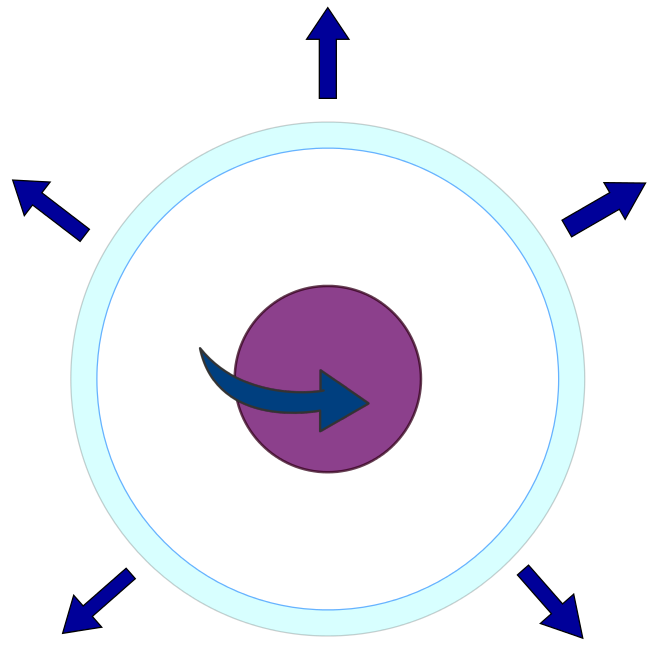
\includegraphics[width=0.3\textwidth]{./figures/model.png}
\end{center}
\caption{\textbf{Model:} A central rotating galaxy surrounded by an expanding thin shell outflow.
\label{fig:model}}
\end{figure}

In order to simulate all the possible cases we set some key parameters
for the program to vary, and some others fixed which are defined by
the characteristics of LAEs. This are chosen as follows.

\subsubsection{Fixed Parameters}

For the first stage there are two fixed parameters: the optical depth
$\tau = 10^8$ and the galaxy rotation velocity $v_{gal}=100$ \kms. For
the second stage there is one fixed parameter: the metallicity of the
outflow $Z=-4.0$. This 3 fixed values are selected because the
characteristics of observed LAEs, especially their low mass and their
highest star formation rate of all. 

\subsubsection{Free Parameters}

We have then 3 parameters left that are going to vary along a wide
range. These are: the galaxy viewing angle \ang, the hydrogen column
density \nh and the outflow expanding velocity \vel. 

\ang covers 3 different angles: $0^\circ$, $45^\circ$ and
$90^\circ$. \lognh takes 41 different values from 20.0 to 22.5. And
\vel covers 5 equidistant velocities from 100 \kms to 500 \kms. The
permutations of these three are analyzed in section
\ref{sec:results}. 


\section{Results}
\label{sec:results}

The results of this project consist of emulating a LAE spectrum basing on its physical characteristics defined by the 3 free parameters we stated before. When defined the combination of those three. \\

---------------------------------------------------------------------\\
MISSING: \\
- What are the compact results.\\
- Not a physical analysis yet. \\
- Write better (prettier)\\
-----------------------------------------------------------------------\\

In the following subsection each free parameter is explained deeper. \\

\subsection{Influences of the Free Parameters}

In order to study the influence of each of the three free parameters, we fix two of them and see how the final spectrum varies along the other one left. In each case we will state these changes.

\subsubsection{Influence of the Galaxy Viewing Angle: \ang}

If one sets fixed outflow \vel and \lognh in each case the viewing angle has the same effect: it increases proportionally the intensity. However this change is not that significant. The resulting spectra are completely the same, but enlarged vertically by a small factor. Fig. \ref{fig:influence_ang} helps visualize this effect in a better way.

\begin{figure}[h!]
\begin{center}
  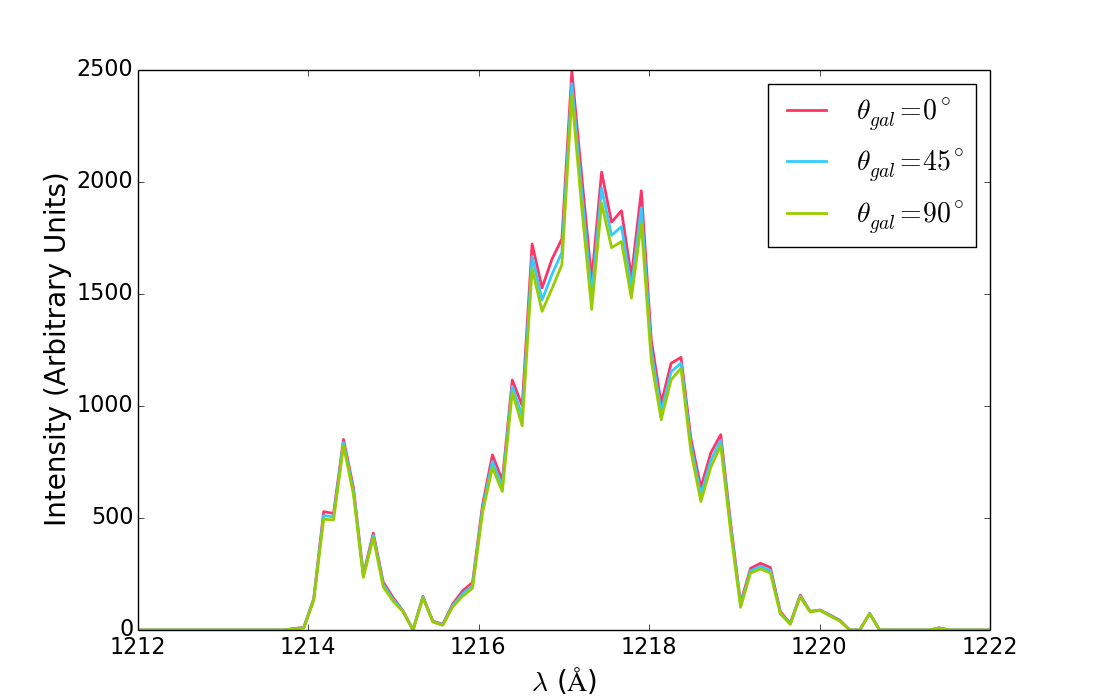
\includegraphics[width=0.5\textwidth]{./figures/influence_ang.png}
\end{center}
\caption{\textbf{Influence of Galaxy Viewing Angle:} The values of the fixed parameters are \vel = 100 \kms and \lognh = 21.3125. The 3 possible angles are shown in the plot with different colors. The increase is visible as well as its small enlargement factor.\\
\label{fig:influence_ang}}
\end{figure}

\subsubsection{Influence of the Outflow Hydrogen Column Density: \lognh }

The effect of the \lognh is the creation of 2 peaks: the left one very thin, tall and pronounced, and the right one very wide, small and soften. When the $log{nH}$ is increased, the left peak starts to decrease while mixing with the right one, decreasing their height ratio until the left peak completely disappears. The resulting spectrum, with high column density, is a wide single mountain with intensity significantly less than at the beginning. Fig. \ref{fig:influence_lognH} helps visualize this effect in a better way.

\begin{figure}[h!]
\begin{center}
  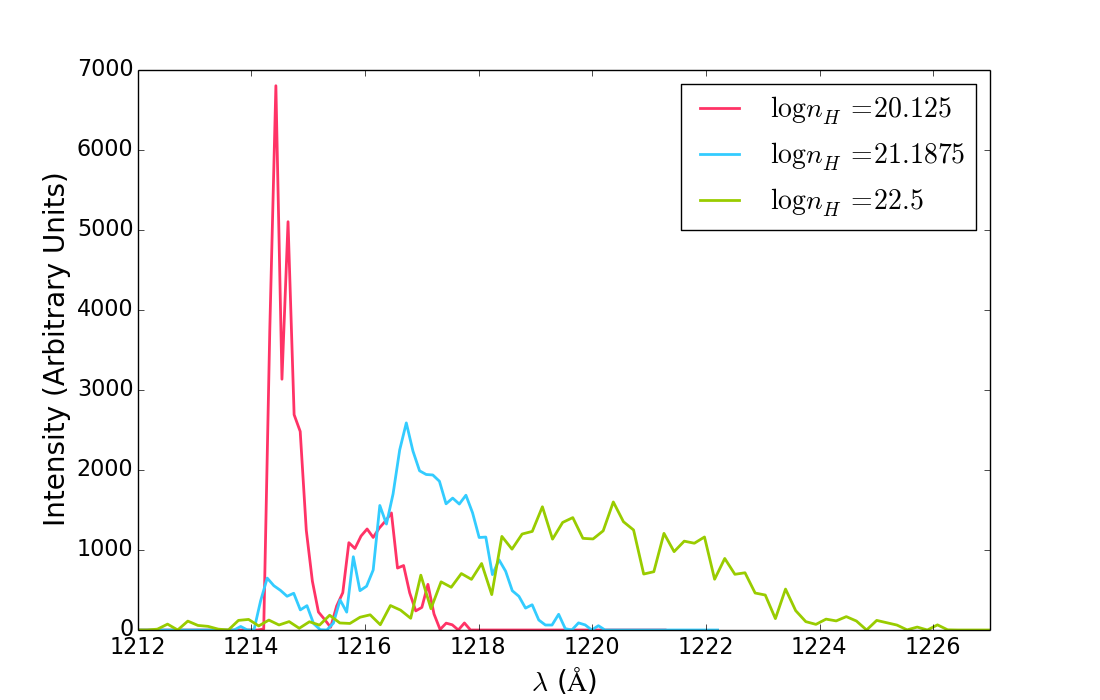
\includegraphics[width=0.5\textwidth]{./figures/influence_lognH.png}
\end{center}
\caption{\textbf{Influence of Outflow Hydrogen Column Density:} The values of the fixed parameters are \vel = 100 \kms and \ang = 90$^\circ$. There are three stages of the \lognh value shown: initial, intermediate and final, with the values shown on the plot.\\
\label{fig:influence_lognH}}
\end{figure}

\subsubsection{Influence of the Outflow Expanding Velocity: \vel }

The effect of this parameter consists in a shift of the initial spectrum in the column density. The more \vel the outflow has, the more the spectrum simulates the previous velocity but with a greater \lognh. If one compares with Fig. \ref{fig:influence_lognH} the similarities are really clear. 

\begin{figure}[h!]
\begin{center}
  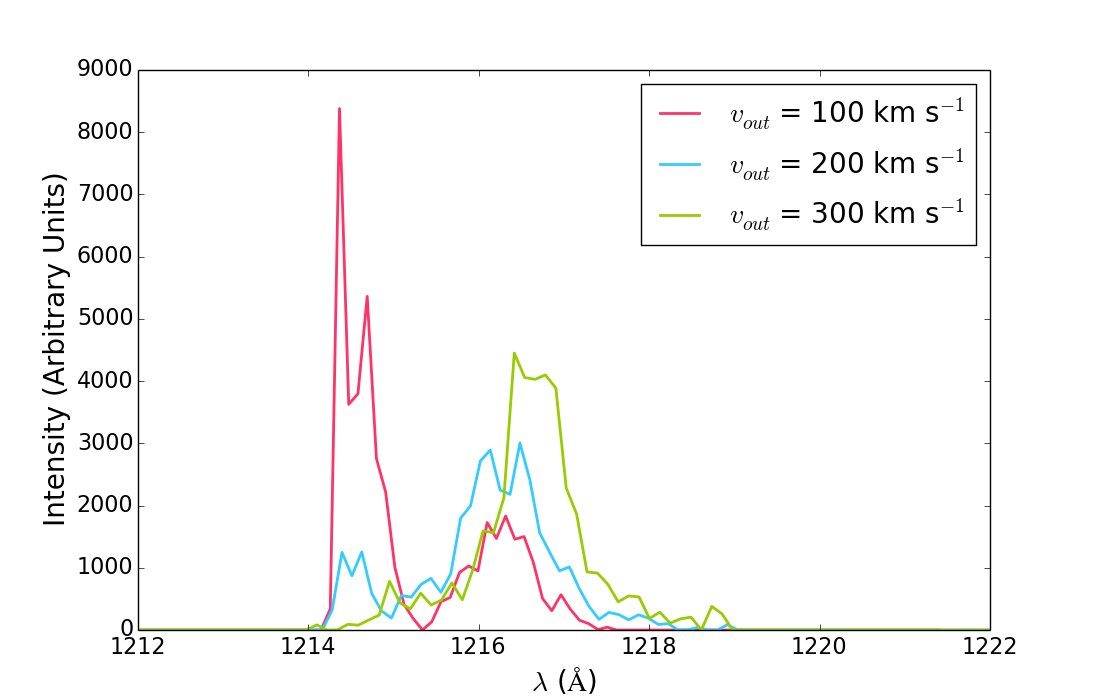
\includegraphics[width=0.5\textwidth]{./figures/influence_vel.png}
\end{center}
\caption{\textbf{Influence of Outflow Expanding Velocity:} The values of the fixed parameters are \lognh = 20.0625 and \ang = 90$^\circ$. If one increases \lognh for an outflow with \vel = 100 \kms it will create similar spectra to these in certain points.\\
\label{fig:influence_vel}}
\end{figure}


\section{Discussion}
\label{sec:discussion}

---------------------------------------------------------------------\\
MISSING: \\
- Comparison with some other result (probably observations).\\
- Why is this result useful? \\
- What possible implications can this model have?\\
-----------------------------------------------------------------------\\

Ideas: \\

The decrease of the intensity while increasing the column density is caused because the second is proportional to the absorption of light in the gas. The more \lognh, the less photons get out of the outflow.

\section{Conclusions}
\label{sec:conclusions}
Here goes the conclusions....

\section*{Acknowledgments}

We acknowledge Alvaro Orsi and Julian Mejia for collaborating with us offering their time, advice and especially data. We used their outflow simulations in order to get our results.\\

The data, source code and instructions to replicate the results of this paper can be found here {\texttt{https://github.com/mariacamilaremolinagutierrez/ LymanAlpha/}}.
Most of our code benefits from the work of the IPython and Matplotlib communities \citep{IPython,matplotlib}.\\

---------------------------------------------------------------------\\
MISSING: \\
- More acknowledgments.\\
-----------------------------------------------------------------------\\

\bibliographystyle{latex/apj}
\bibliography{references}

\newpage

%\section{Ejemplos para tener en cuenta}
%
%Ejemplo display math
%
%\begin{displaymath}
%J(x,b,\phi,i)=\frac{\sqrt{\pi}}{\sqrt{24}a\tau_0}\Bigg{(}\frac{(x-x_{\rm
%    b})^2}{1+{\rm cosh}\Big{[}\sqrt{\frac{2\pi^3}{27}}\frac{|(x
%      -x_{\rm b})^3|}{a\tau_0}\Big{]}}\Bigg{)},
%\end{displaymath}
%
%Ejemplo tabla
%
%\begin{table}
%\begin{center}
%\begin{tabular}{c cccccc}
%\hline \hline
%Source & $\tau_{H}$ & &  $\ V_{\rm max}$& & \\
%Distribution& &    & (\kms) & & \\
%& & 0 & 100 &200 & 300\\ \hline
%Homogeneous & $10^{5}$& 0.263 &  0.263 &  0.263 &  0.263  \\
%            & $10^{6}$ & 0.291 &   0.292 &  0.293 &  0.293 \\
%Central & $10^{5}$ &  0.096 & 0.096 &  0.096 & 0.096 \\
%  		&$10^{6}$ & 0.066 &  0.066 &  0.066 &  0.066 \\
%\hline
%\end{tabular}
%\caption{
% Ejemplo de tabla. }
%\label{table:escape}
%\end{center}
%\end{table}

\end{document}
